\documentclass[a4paper,12pt]{article}

\usepackage[top=2cm, bottom=2cm, left=2cm, right=2cm]{geometry}
\usepackage{amsmath}
\usepackage{amssymb}
\usepackage{graphicx} 
\usepackage{caption}
\usepackage{dsfont}
\usepackage{verbatim}
\usepackage{pdfpages}
\usepackage{subfig}

\renewcommand{\thepart}{}
\renewcommand{\thesection}{\arabic{section}}
\renewcommand{\thesubsection}{\arabic{section}.\arabic{subsection}}

%-------------------------------------------------------------------------------
\begin{document}

%Include cover
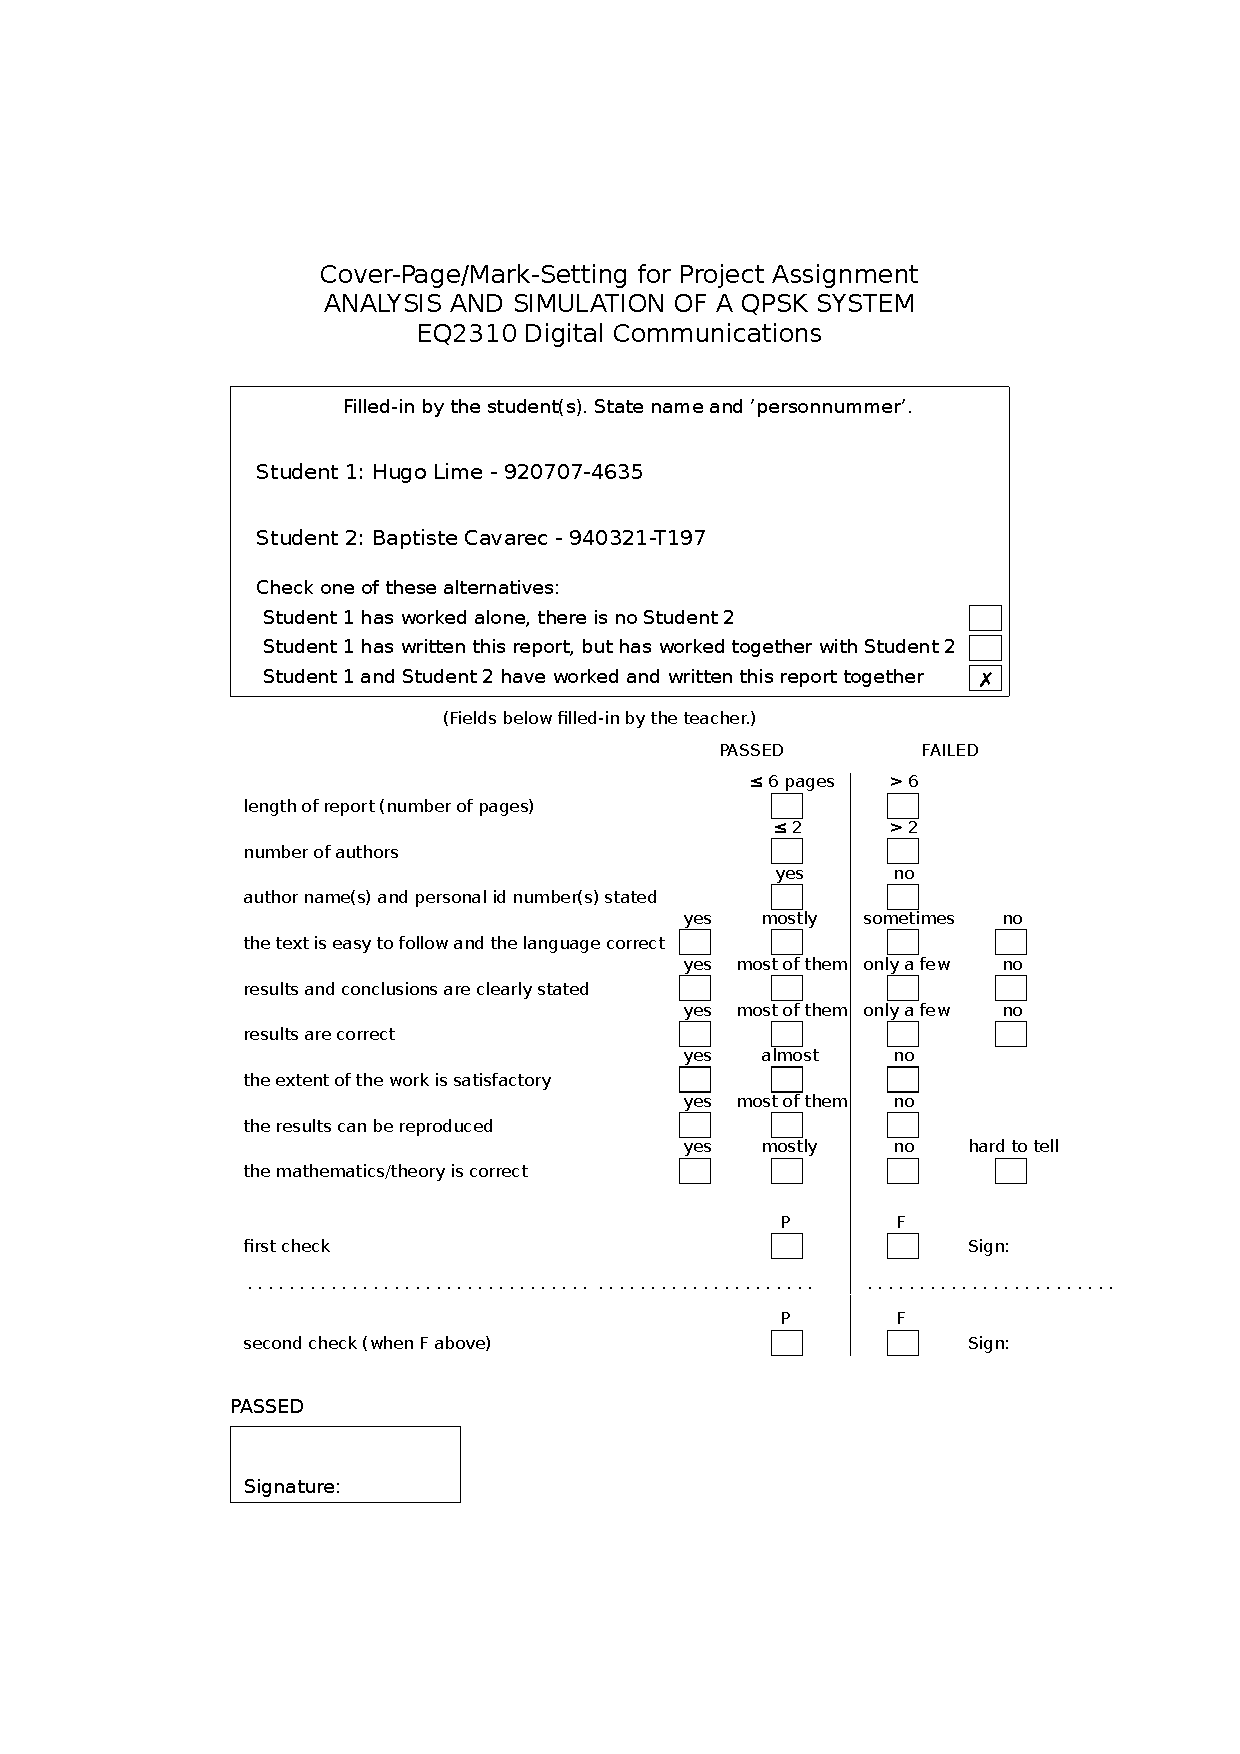
\includepdf[pages={1}]{Cover_filled.pdf}
\newpage

%Abstract
\section*{Abstract}
In this report, we investigate the influence of mutlitple parameters in a simulated QPSK radio communication channel.
First, we show how the bit error rate varies with the signal-to-noise ratio in a perfectly synchronized environment. Then we study how synchronization and phase estimation modify the BER, how theses algorithms behave under AWGN and how they are influenced by the training sequence.

%-----------------------------------------------------------------------------------
%Partie 1
\section{Ideal Bit Error Rate (BER) performances}

\subsection{Exact expression}
\begin{figure}[ht!]
\centering
\begin{center}
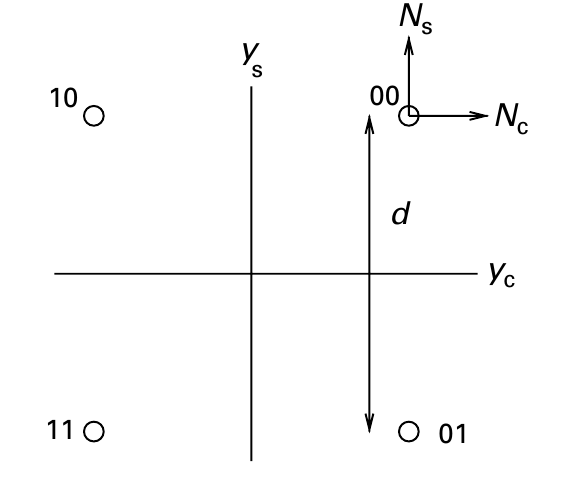
\includegraphics[scale=0.20]{Gray_coded_QPSK.png}
\caption{Gray coded bitmap from \cite{Madhow}}
\end{center}
\end{figure}
The exact expression of the BER can easily be derived as:
\begin{equation}
p_{b}=Q(\sqrt{\frac{2E_{b}}{N_{0}}})
\end{equation}

\subsection{Simulation results and comparison}
In order to simulate a environment with perfect synchronization, we forced the value of $t_{samp}$ which equals to the samples coming from the guards bits and the delay caused by the matched filter. The phase offset is set to $0$.
\begin{figure}[ht!]
\centering
\begin{center}
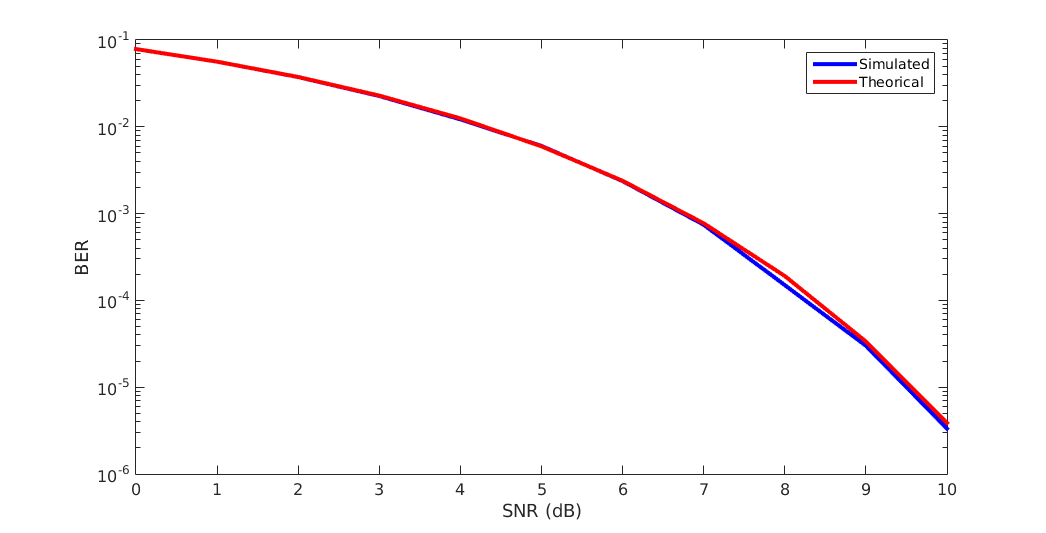
\includegraphics[scale=0.30]{BER_Exact-Sim.png}
\caption{BER comparison}
\label{BER}
\end{center}
\end{figure}
As shown in Figure \ref{BER}, the simulated values are very similar to the theorical ones. However, for very high SNR, the BER is so small that our testing set (here 300 blocks of 1000 data bits) is not large enough to be relevant.

%-----------------------------------------------------------------------------------
%Partie 2
\newpage
\section{Non-ideal synchronization and phase estimation}
\subsection{Influence of time and phase estimation on the BER}
For a SNR of $5dB$, we created errors in synchronization and phase estimation to see how it modifies the BER.

\begin{figure}[ht]
\begin{minipage}[c]{.45\linewidth}
\begin{center}
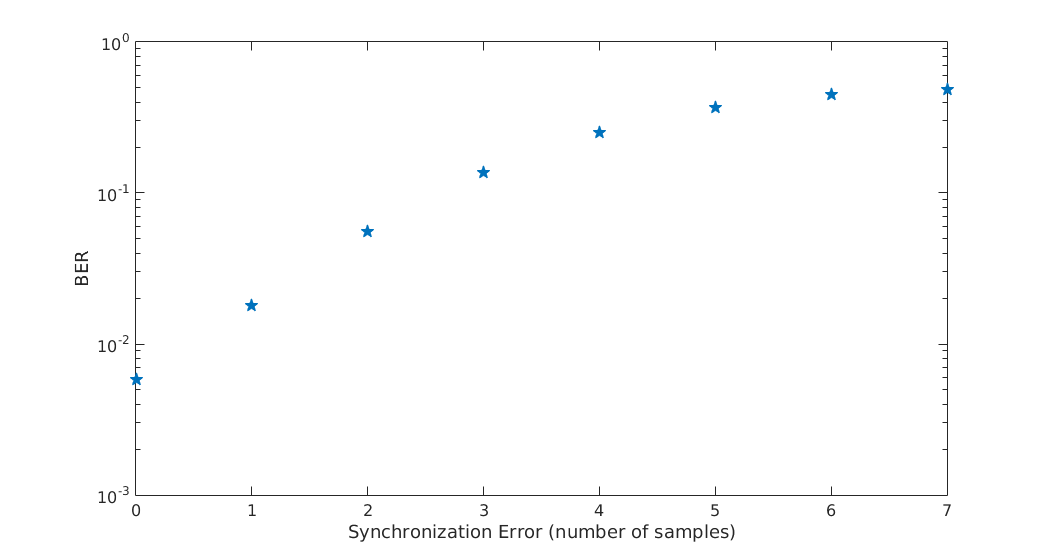
\includegraphics[scale=0.35]{BER_SyncError.png}
\caption{BER with synchronization errors}
\label{BER_sync}
\end{center}
\end{minipage}
\hfill
\begin{minipage}[c]{.45\linewidth}
\begin{center}
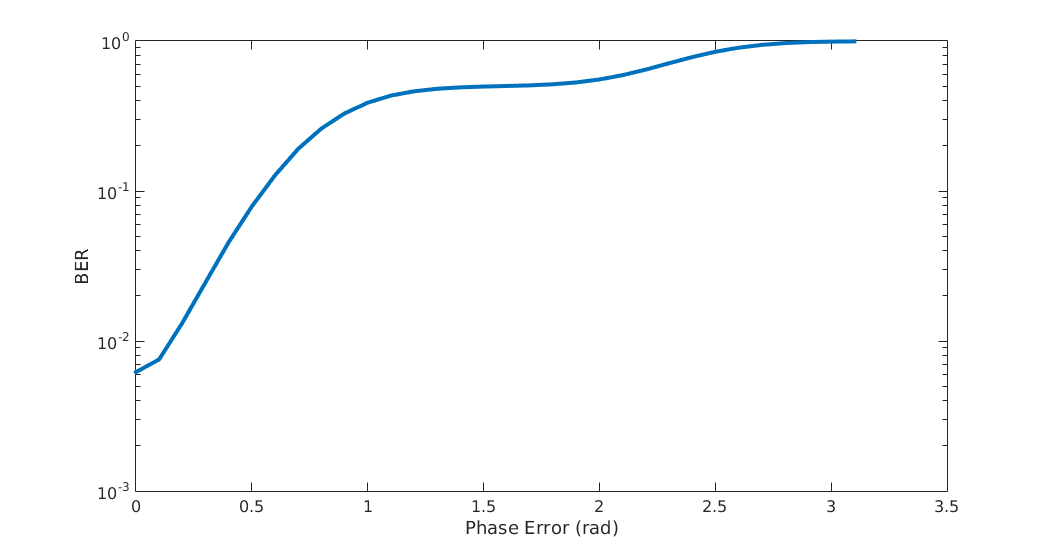
\includegraphics[scale=0.35]{BER_PhaseError.png}
\caption{BER with phase errors}
\label{BER_phase}
\end{center}
\end{minipage}
\end{figure}

Figure \ref{BER_sync} shows that one single error in the synchronization is catastrophic, the BER is multiplyed by 2. With a shift of 2 samples, the BER is 10 times higher.\\

Figure \ref{BER_phase} shows that phase estimation can greatly increase the BER. However, for small error (typically less than 0.1 rad) the loss is acceptable. To better understand the influence of a phase error on the BER, we can look at the constellation on Figure \ref{Constellation}. We can see that when we increase the noise power, a lot of samples are detected near a border of a decision region. Therfore, a phase estimation error can easily put the sample in a wrong region.

\begin{figure}[ht]
\subfloat[$SNR=0$]{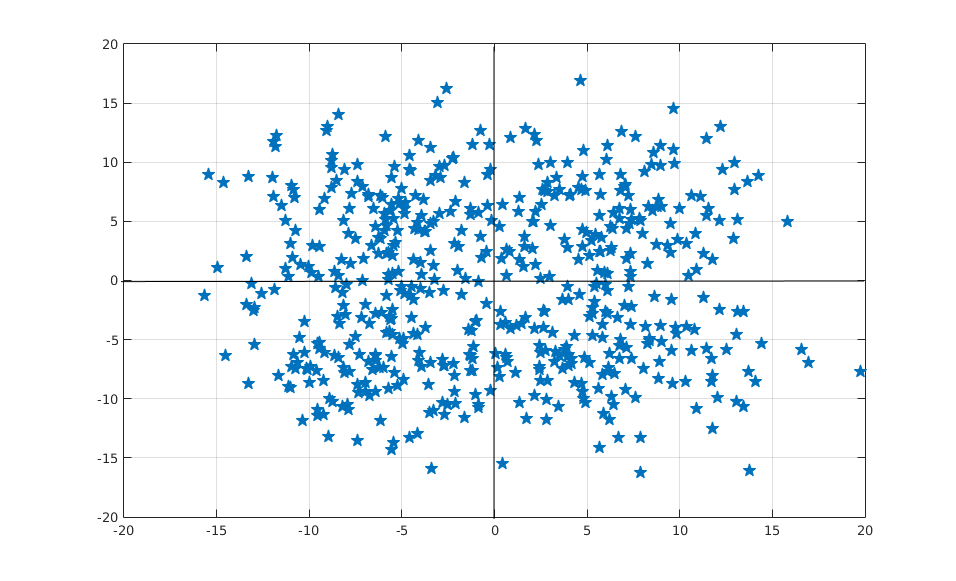
\includegraphics[width=0.35\textwidth]{Constellation_SNR0.png}} 
\subfloat[$SNR=5$]{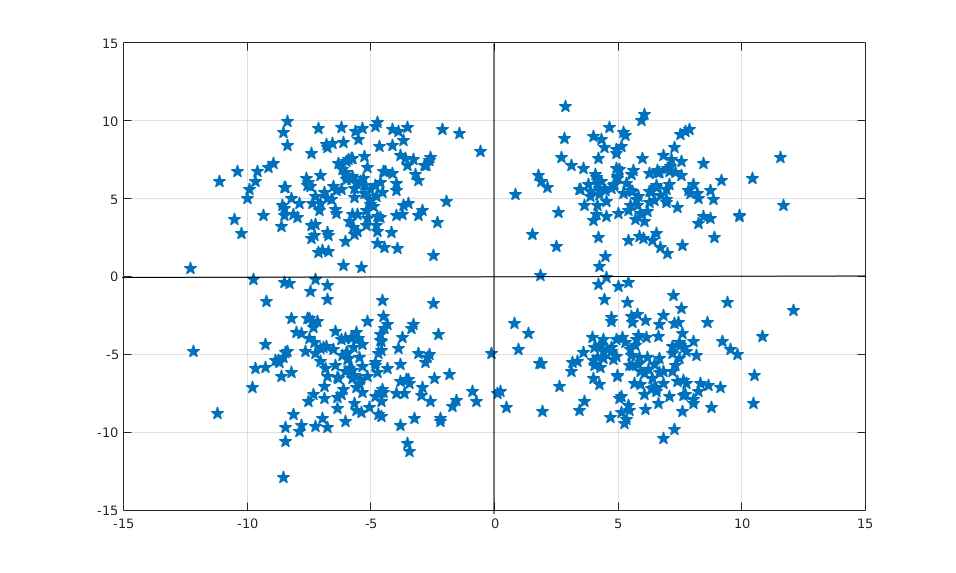
\includegraphics[width=0.35\textwidth]{Constellation_SNR5.png}} 
\subfloat[$SNR=10$]{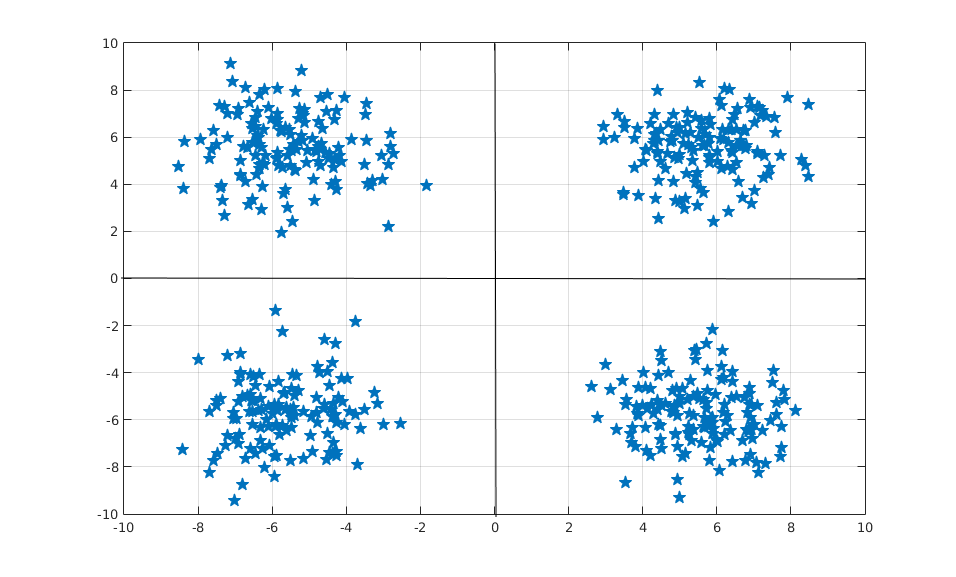
\includegraphics[width=0.35\textwidth]{Constellation_SNR10.png}} 
\caption{Constellation Diagrams}
\label{Constellation}
\end{figure}


\subsection{Synchronization and phase estimation under AWGN}
We implemented the recommanded synchronization algorithm (maximum cross-correlation between the filtered signal and a copy af the training sequence). Figure \ref{SE} shows that this algorithm is very resilient to the noise, for a reasonable SNR errors never occur. However, one should take into account that we used a small window (around 6 symbols) centered on the real value. In a real environment we would need another sytem to position the window (like a power detector). \\

In order to estimate the phase, we searched for the angle that would minimize the norm of the difference between the rotated signal and the training sequence. We can see on Figure \ref{SE} that the estimate is quite sensible to noise. But, as stated before, a phase error of less than 0.1 rad has a resonable effect on the BER. It could be improved by using another algorithm, or a phase-locked loop.


\begin{figure}[ht]
\begin{minipage}[c]{.45\linewidth}
\begin{center}
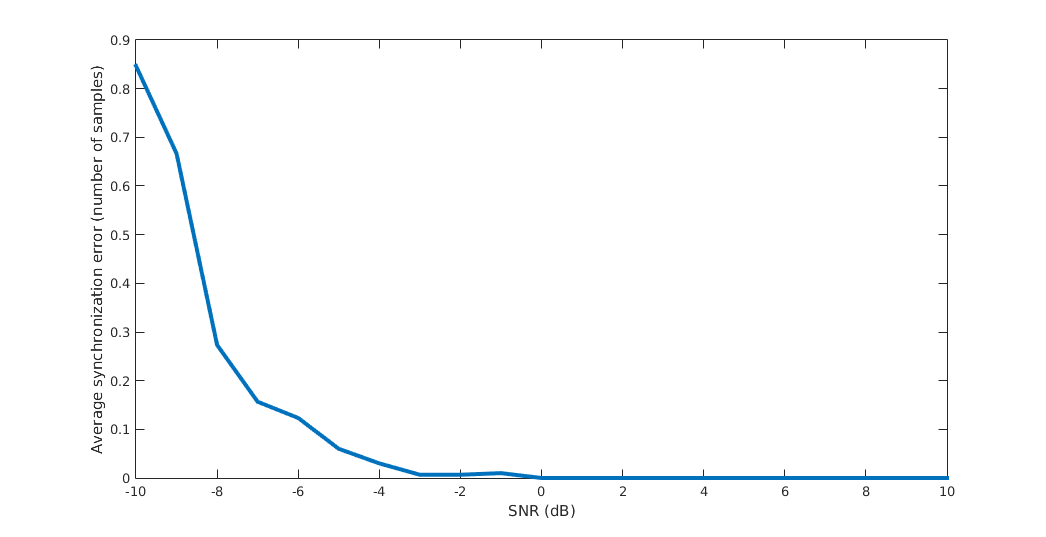
\includegraphics[scale=0.35]{SynError.png}
\caption{time estimation error}
\label{SE}
\end{center}
\end{minipage}
\hfill
\begin{minipage}[c]{.45\linewidth}
\begin{center}
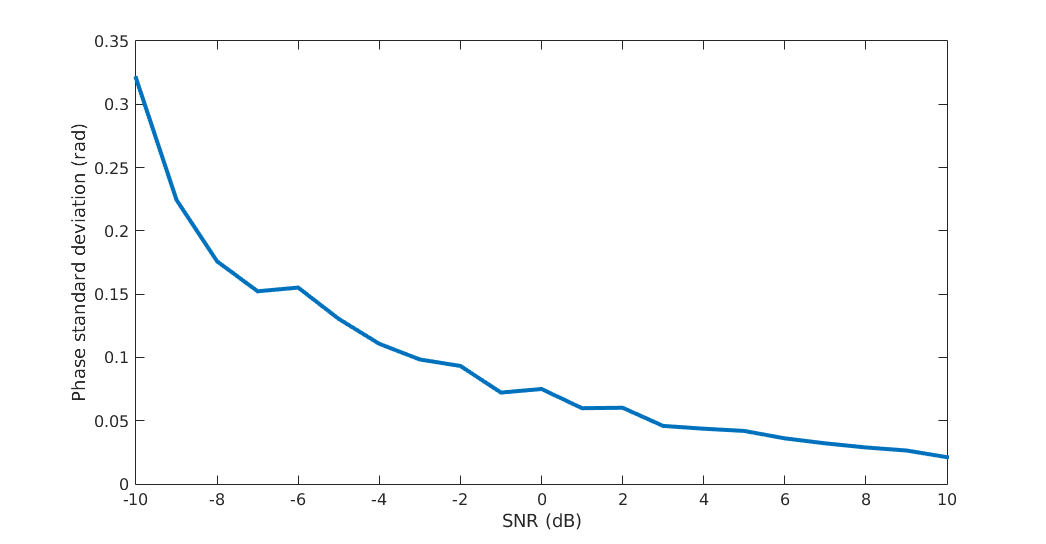
\includegraphics[scale=0.35]{PhaseError.png}
\caption{Phase estimation error}
\label{PE}
\end{center}
\end{minipage}
\end{figure}

\subsection{Influence of the training sequence}
We computed the synchronization and phase estimation errors when changing the number of training bits at a fixed SNR of 0. Figure \ref{TSE} shows that with a training sequence of more than 20 bits, we have less than 10\% chance of having a synchronization error.\\

For the phase estimation, if we want less than 0.1 rad deviation as we concluded before, we need at least 50 training bits. With a fixed sequence of 1000 data bits, this would corresponds to a 5\% overhead.

\begin{figure}[ht]
\begin{minipage}[c]{.45\linewidth}
\begin{center}
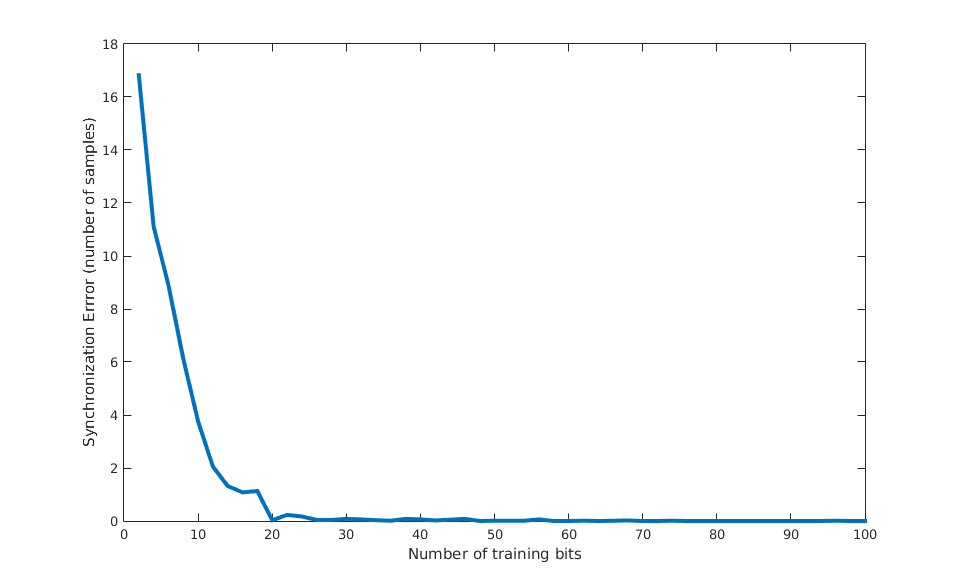
\includegraphics[scale=0.35]{Training_sync.png}
\caption{time estimation error}
\label{TSE}
\end{center}
\end{minipage}
\hfill
\begin{minipage}[c]{.45\linewidth}
\begin{center}
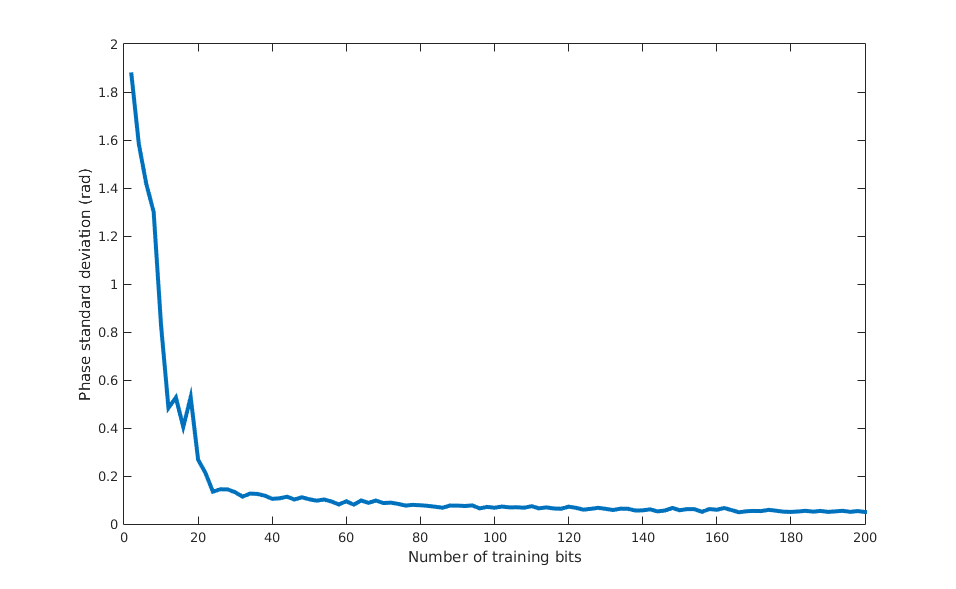
\includegraphics[scale=0.35]{Training_phase.png}
\caption{Phase estimation error}
\label{TPE}
\end{center}
\end{minipage}
\end{figure}

To improve the training sequence, we need to find one that has an autocorrelation function that is similar to a Dirac. To do this, we tested a number of random training sequences for which we computed its autocorrelation function. Then we chose the one that had the autocorrelation function most similar to a Dirac. Figure \ref{train} shows that for a small training sequence it can improve a little the performances of the synchronization.

\begin{figure}[ht!]
\subfloat[10 bits]{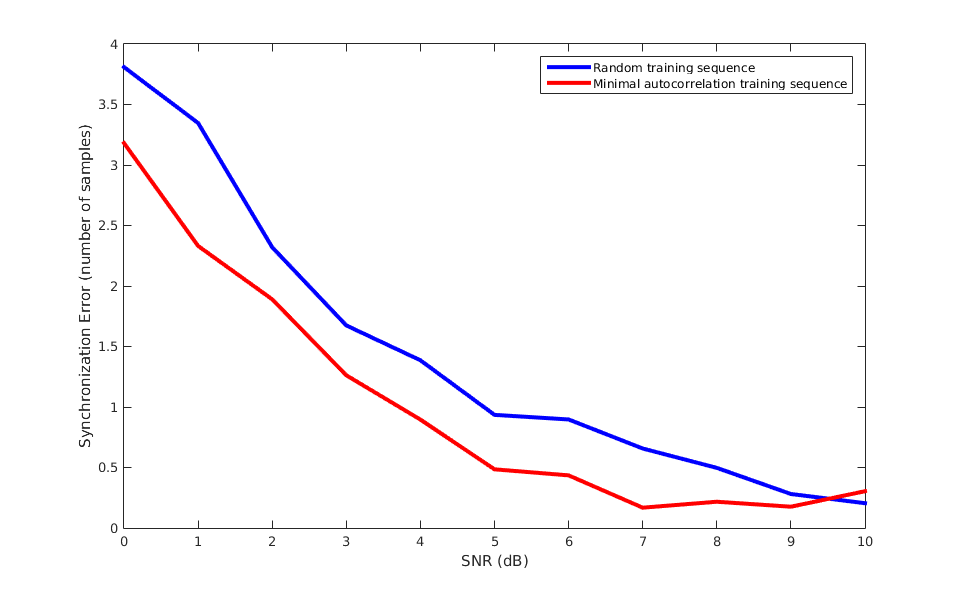
\includegraphics[width=0.55\textwidth]{Training_seq10.png}} 
\subfloat[20 bits]{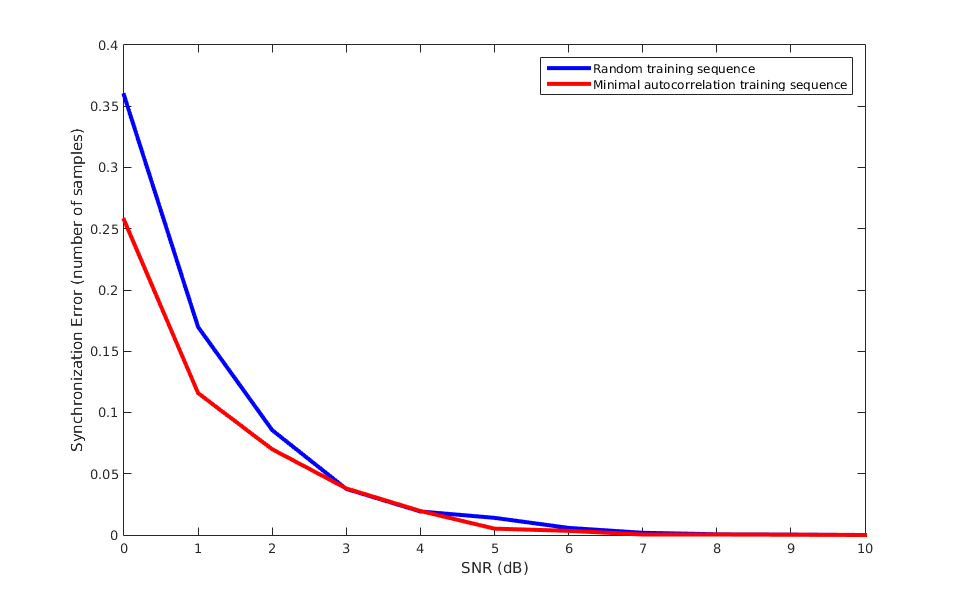
\includegraphics[width=0.55\textwidth]{Training_seq20.png}}  
\caption{Difference between random and chosen training sequence}
\label{train}
\end{figure}

%-----------------------------------------------------------------------------------
%Partie 2
\newpage
\section{Differential modulation}


%---------------------------------------------------------------------------------
%Conclusion
\section*{Conclusion}
\vspace{1cm}
jflsdjqfmljqskldj

%---------------------------------------------------------------------------------------
%Appendix
\appendix

%References
\bibliographystyle{plain}
\bibliography{report_biblio}

%------------------------------------------------------------------------------------
%Matlab code
\clearpage
\renewcommand{\thesubsection}{\arabic{subsection}}
\section*{Matlab Code}
\setcounter{subsection}{0}
\subsection{Detect.m}
\begin{verbatim}
CODE
\end{verbatim}






%---------------------------------------------------------------------------------------------------------
\end{document}